\section*{File Transfer Protocol (FTP)}
Es uno de los protocolos estandar del Internet, utilizados para transferir archivos de datos entre un cliente y un servidor. Fue desarrollado a principios de los 70s por Abhay Bhushan (MIT). Se creó inicialmente para permitir la transferencia segura entre servidores y computadores del ARPANET.
\subsection*{Funcionamiento}
Tiene una arquitectura cliente/servidor proporcionando servicio a travez  de dos puertos:
\begin{itemize}
\item \texttt{Port: 20} Para la transferencia de datos
\item \texttt{Port: 21} Para control (órdenes)
\end{itemize}
El cliente se conecta al servidor desde un puerto superior al 1024 y hace una solicitud al servidor por el \texttt{Port: 21}, que siempre está escuchando als peticiones de los clientes por ese puerto. Una vez establecido se pueden usar las ordenes especificas.
\subsubsection*{Usuarios}
\begin{itemize}
\item \textbf{Autentificados:} Ingresan con nombre y contraseña. Dentro de estos, hay usuarios \texttt{FTP} y virtuales.  Los primeros son usuarios del sistema y pueden acceder a partes del sistema con permisos. Los virtuales son los que tienen cuentas en BD como MySQL y solo se autentifican para utilizar \texttt{FTP}.
\item \textbf{Anónimos:} No disponen de cuenta y para conectarse al servidor \texttt{FTP} introducen cuentas simbólicas. Es la forma convencional de llamar al servicio de transferencia de ficheros que las organizaciones dejan para acceso público. La clave mas habitual es \texttt{guest}.
\end{itemize}
\subsection*{Modos de Conexión a un Servidor FTP}
\noindent
\begin{minipage}[t]{.5\textwidth}
\raggedright
\subsubsection*{Modo Activo}
\begin{enumerate}
\item El cliente se conecta desde un puerto de control aleatorio superior al 1024 (en nuestro caso el 1035) al puerto de control del servidor, puerto 21. El cliente empieza a escuchar por el puerto 1036 y envía este puerto de control al servidor.

\item El servidor responde con un ACK al puerto de control del cliente.

\item El servidor inicia una conexión entre su puerto de datos (puerto 20) y el puerto de datos del cliente (puerto 1036)

\item El cliente responde con un ACK al servidor.
\end{enumerate}    
\end{minipage}% <---------------- Note the use of "%"
\begin{minipage}[t]{.5\textwidth}
\raggedright
\subsubsection*{Modo Pasivo}
\begin{enumerate}
\item El cliente se conecta desde un puerto de control aleatorio superior al 1024 (en nuestro caso el 1035) al puerto de control del servidor, puerto 21. El cliente envía un comando PASV al servidor.

\item El servidor responde con un ACK, desde un puerto aleatorio superior al 1024 (en nuestro caso el 2040) al puerto de control del cliente.

\item El cliente inicia una conexión entre su puerto de datos del cliente (puerto 1036) y el puerto de datos del servidor (puerto 2040)

\item El servidor responde con un ACK al cliente.
\item Cerrar sesión.
\end{enumerate}
%\begin{center}
%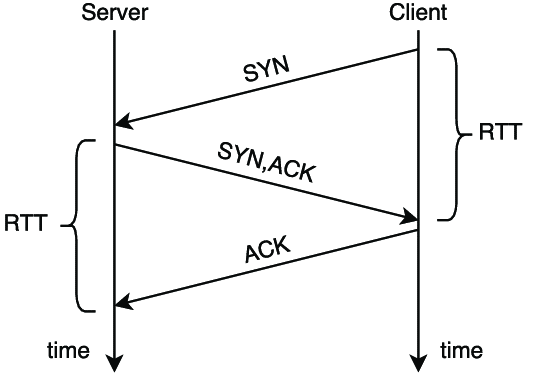
\includegraphics[scale=0.45]{3WAY.png}
%\end{center}
\end{minipage}


\noindent
\begin{minipage}[t]{.5\textwidth}
\raggedright
   \begin{figure}[H]                           
\centering                                  
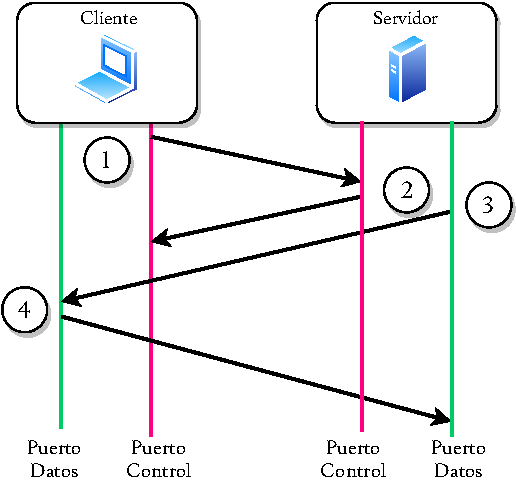
\includegraphics[page=1,scale=0.7]{Activo.pdf}
\caption{Activo} 
\end{figure}    
\end{minipage}% <---------------- Note the use of "%"
\begin{minipage}[t]{.5\textwidth}
\raggedright
\begin{figure}[H]                           
\centering                                  
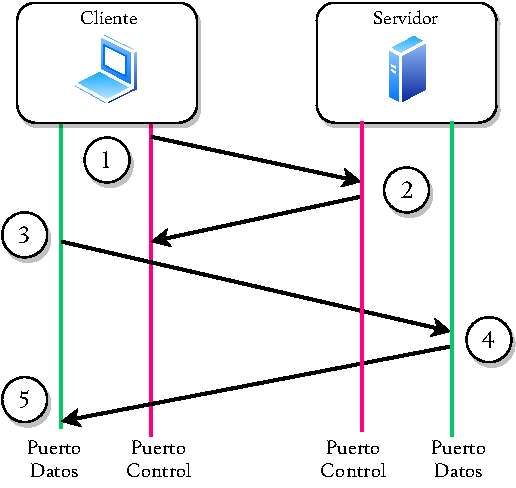
\includegraphics[page=1,scale=0.7]{Pasivo.pdf}
\caption{Pasivo} 
\end{figure}    
\end{minipage}
 \subsection*{Modos de Transferencia}
\begin{itemize}
\item Modo \texttt{ASCII}: Se usa para transmitir texto y \texttt{HTML}.
\item Modo Binario: Transfiere zips, imagenes, ejecutables. No se pueden enviar en modo \texttt{ASCII} ya que causarian problemas y viceversa.
\end{itemize}
\subsection*{Servidores FTP}
Algunos servidores FTP.
\begin{itemize}
\item \textbf{Cerberus FTP Server:} Propietario, Windows. FTP, FTPS, SFTP, SCP, cliente web HTTPS, IPv6, API de servicios web basados en SOAP, autenticación de Windows Active Directory / LDAP, administración remota HTTP / HTTPS, clave pública y autenticación de certificado de cliente
\item \textbf{CrushFTP Server:} Trialware, Mac, Windows, Linux. FTP, FTPS, SFTP, SCP, HTTP, HTTPS, WebDAV (SSL), AS2, AS3, API de complemento, autenticación de Active Directory / LDAP, autenticación RADIUS, autenticación SQL, autenticación SSL SAML, equilibrador de carga CrushBalance, administración de IU web, grupos, Herencia en capas, eventos / alertas, conversión de protocolo (protocolos entrantes FTP / FTPS / SFTP / HTTP (s) convertidos en un servidor back-end FTP (ES) / SFTP / HTTP (s) / S3 / WebDAV).
\end{itemize}
 \section*{Trivial File Transfer Protocol (TFTP)}
 Es un protocolo de transferencia simple semejante a una version basica de FTP y se utiliza para transferir archivos pequeños.
\subsection*{Características}
\begin{itemize}
\item Utiliza \texttt{UDP} en el puerto 69.
\item No existen mecanismos de autentificación o cifrado.
\item Se utiliza para leer o escribir ficheros en un servidor remoto.
\end{itemize}
Dado que \texttt{UDP} no es confiable, utiliza el tiempo de espera y retransmisión para garantizar que lleguen los datos. El lado emisor transmite un archivo de tamaño fijo (512), espera el \texttt{ACK} del bloque y aguarda un \texttt{ACK} por cada bloque antes de enviar el siguiente.
\subsection*{Funcionamiento}
Una máquina A, que inicia la comunicación, envía un paquete \texttt{RRQ} (Read Request) o \texttt{WRQ} (Write Request) a una maquina B, con el nombre del archivo y el modo de transferencia. B responde con un \texttt{ACK}, que  tambien sirve para informar a A del puerto que en B al que tiene que enviar los paquetes restantes. La maquina origen envia paquetes de datos numerados al destino, excepto el último conteniendo 512\texttt{Bytes}. La del destino le responde con \texttt{ACK}. El paquete final debe contener menos de 512 de datos para indicar que es el último, si el ultimo es de 512\texttt{Bytes} exactos, se envia un siguiente con 0\texttt{Bytes}.

%\begin{figure}[H]
%\centering
%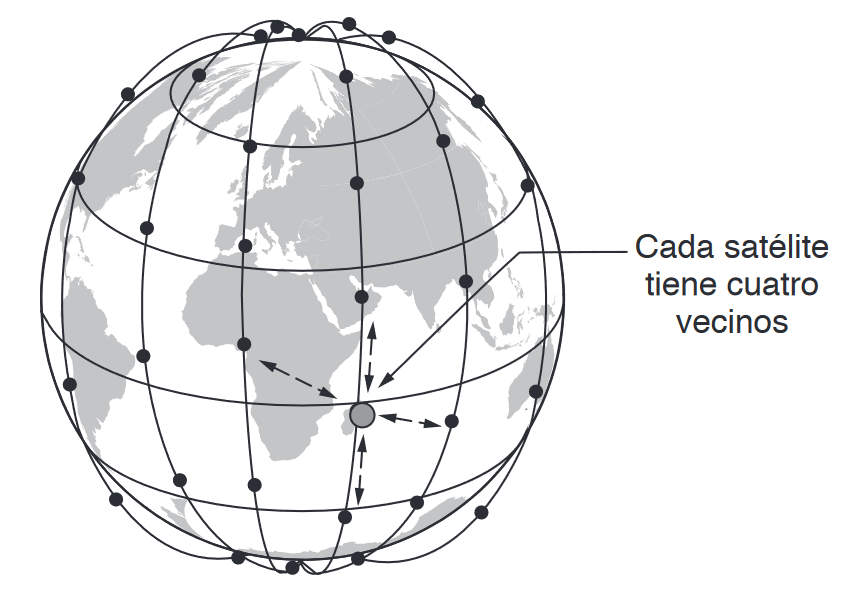
\includegraphics[page=1,scale=0.7]{SATELITES2.png}
%\caption{Satélites Iridium \textit{(Redes de Computadoras, Tanenbaum 4ta Edición, Pagina 105)}}
%\end{figure}

%\begin{figure}[H]
%\centering
%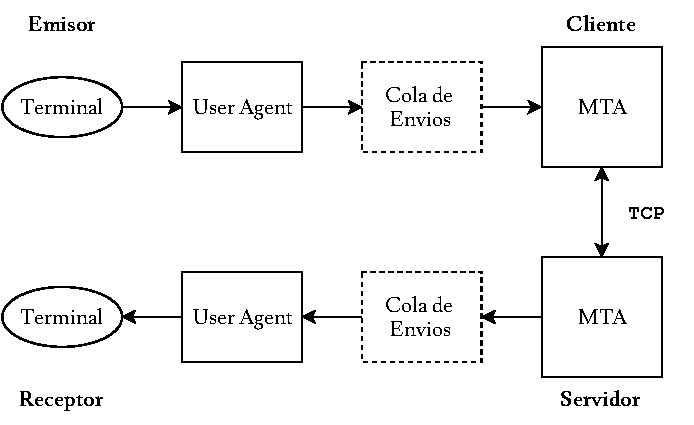
\includegraphics[page=1,scale=0.7]{SMTP.pdf}
%\caption{Esquema de funcionamiento de SMTP}
%\end{figure}
